\documentclass[12pt,xcolor=svgnames]{beamer}
\usepackage{dsfont,natbib,setspace}
\mode<presentation>

% replaces beamer foot with simple page number
\setbeamertemplate{navigation symbols}{}
\setbeamertemplate{footline}{
  \vspace{-1.5cm}
  \raisebox{10pt}{\makebox[\paperwidth]{\hfill\makebox[20pt]{\color{gray}\scriptsize\insertpagenumber}}}}

% colors
\newcommand{\bk}{\color{black}}
\newcommand{\rd}{\color{red}}
\newcommand{\fg}{\color{ForestGreen}}
\newcommand{\mar}{\color{Maroon}}
\newcommand{\org}{\color{Orange}}
\newcommand{\bl}{\color{blue}}
\newcommand{\gr}{\color{gray}}
\newcommand{\theme}{\color{FireBrick}}
\newcommand{\fb}{\color{FireBrick}}
\newcommand{\hlf}{\setstretch{1}}

% common math markups
\newcommand{\bs}[1]{\boldsymbol{#1}}
\newcommand{\mc}[1]{\mathcal{#1}}
\newcommand{\mr}[1]{\mathrm{#1}}
%% \newcommand{\bm}[1]{\mbox{\boldmath $#1$}}
\newcommand{\bm}[1]{\mathbf{#1}}
\newcommand{\mb}[1]{\mathbf{#1}}
\newcommand{\ds}[1]{\mathds{#1}}

% spacing and style shorthand
\newcommand{\sk}{\vspace{.4cm}}
\newcommand{\nochap}{\vspace{0.5cm}}
\newcommand{\nsk}{\vspace{-.4cm}}
\newcommand{\chap}[1]{{\theme \Large \bf #1} \sk}
\newcommand{\R}[1]{{\bl\tt #1}}
\newcommand{\til}{{\footnotesize$\bs{\stackrel{\sim}{}}$ }}

% specific stats markups for this doc
\newcommand{\E}{\ds{E}}
\newcommand{\Reals}{\ds{R}}
\newcommand{\var}{\text{var}}
\newcommand{\cov}{\text{cov}}
\newcommand{\mT}{\mc{T}}
\newcommand{\GP}{\mc{GP}}
\newcommand{\iidsim}{\stackrel{\mathrm{iid}}{\sim}}
\newcommand{\indsim}{\stackrel{\mathrm{ind}}{\sim}}
\newcommand{\mN}{\mc{N}}

\usepackage{graphicx}
\graphicspath{{graphics/}}

\begin{document}

{ \usebackgroundtemplate{}%\includegraphics[height=\paperheight]{phoenix}}
\thispagestyle{empty}
\setcounter{page}{0}

\title{\theme \Large \vskip 0.5cm
{\bf VectorBiTE Training 2019 \\ Workshop}\\
\bigskip
\bf {\sf \gr Introduction to Autocorrelated Data \\ and Time Series}}

\author{
\begin{center}

\includegraphics[scale=0.05,trim=10 10 0 150]{VB_logo.jpg}
\end{center}
\texttt{\rd\small www.vectorbite.org}
%Dependent data and autocorrelation, Autoregressive (AR) models , trending and
%     periodic regression models
%\vskip 1cm {\bf Leah R.~Johnson}\\ 
%{\org Virginia Tech}, Statistcs\\
%  \vskip .5cm \texttt{\rd\small leah.johnson-gramacy.com/QED/teaching}
}
\date{}
\maketitle 
}





% doc spacing
\setstretch{1.1}

\begin{frame}
\chap{Time series data and dependence}

Time-series data are simply a collection of observations
gathered over time.
For example, suppose $y_1, \ldots, y_T$ are
\begin{itemize}
\item  daily temperature,
\item  solar activity,
\item  CO$_2$ levels,
\item  GDP,
\item  yearly population size.
\end{itemize}

\sk
{\bl In each case, we might expect what happens at time $t$ to be
correlated with time $t-1$.}

\end{frame}

\begin{frame}


Suppose we measure temperatures, daily, for several years.

\sk
Which would work better as an estimate for today's temp:
\begin{itemize}
\item The average of the temperatures from the previous year? 
\item The temperature on the previous day? 
\end{itemize}

\sk
Would this change if the readings were {\bl iid $\mN(\mu, \sigma^2)$}?


\end{frame}


\begin{frame}
Suppose we measure temperatures, daily, for several years.

\sk
Which would work better as an estimate for today's temp:
\begin{itemize}
\item The average of the temperatures from the previous year? 
\item The temperature on the previous day? 
\end{itemize}

\sk
Would this change if the readings were {\bl iid $\mN(\mu, \sigma^2)$}?

\sk {\rd
Correlated errors require fundamentally different techniques.}

\end{frame}

\begin{frame}[fragile]
\nochap

\vspace{-0.2cm}
{\bl Example:} $Y_t = $ average daily temp.~at O'Hare, Jan-Feb 1997.

{\bl \footnotesize
\begin{verbatim}
> weather <- read.csv("weather.csv")
> plot(weather$temp, xlab="day", ylab="temp", type="l", 
+   col=2, lwd=2)
\end{verbatim}
}

\begin{center}
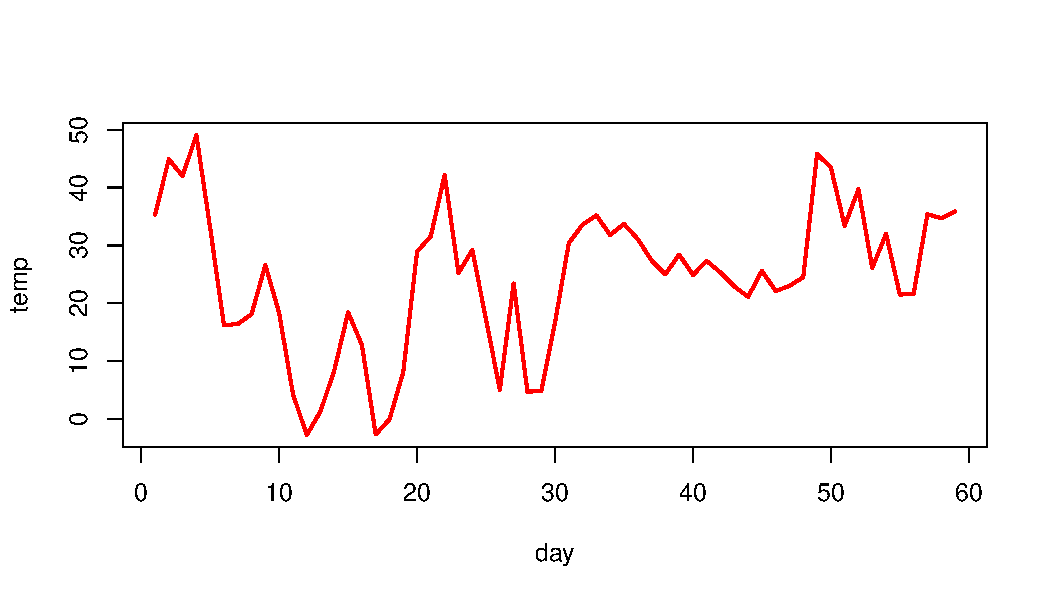
\includegraphics[scale=0.58,trim=10 20 0 55]{weather_new}
\end{center}

\nsk
\begin{itemize}
\item ``sticky'' sequence: today tends to be close to yesterday.
\end{itemize}

\end{frame}


\begin{frame}[fragile]
\nochap

{\bl Example:} $Y_t = $ monthly U.S. beer production (Mi/barrels).

{\bl \footnotesize
\begin{verbatim}
> beer <- read.csv("beer.csv")
> plot(beer$prod, xlab="month", ylab="beer", type="l", 
+   col=4, lwd=2)
\end{verbatim}
}

\begin{center}
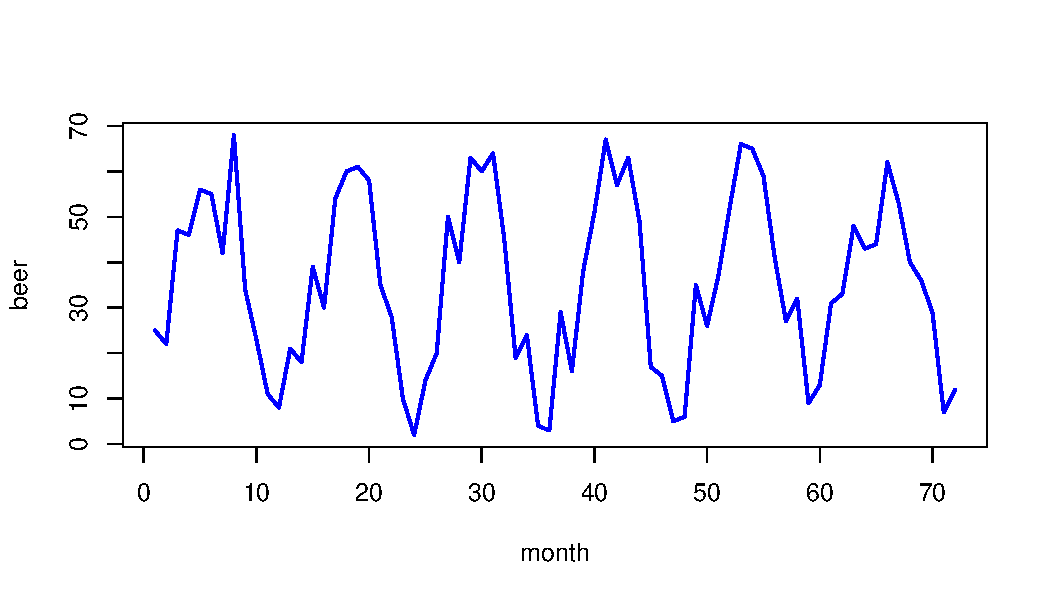
\includegraphics[scale=0.58,trim=10 20 0 55]{beer_new}
\end{center}

\nsk
\begin{itemize}
\item The same pattern repeats itself year after year.
\end{itemize}

\end{frame}


\begin{frame}[fragile]
\nochap


{\bl \small
\begin{verbatim}
> plot(rnorm(200), xlab="t", ylab="Y_t", type="l", 
+   col=6, lwd=2)
\end{verbatim}
}

\begin{center}
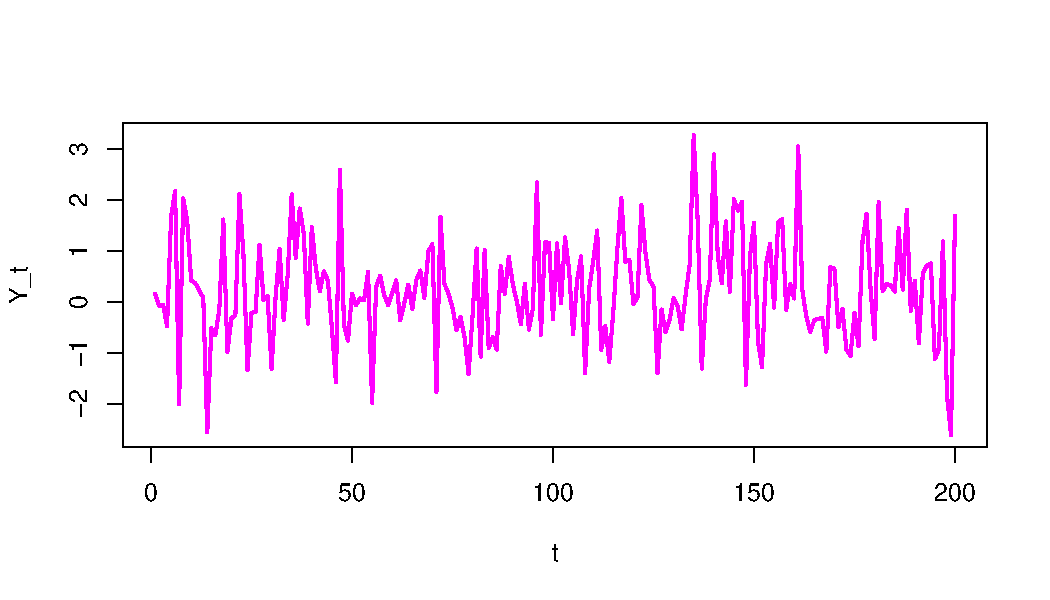
\includegraphics[scale=0.6,trim=10 20 0 55]{norm_new}
\end{center}

\nsk
\begin{itemize}
\item It is tempting to see patterns even where they don't exist. {\bl How do we check?}
\end{itemize}


\end{frame}

\begin{frame}
\chap{Checking for dependence}


To see if $Y_{t-1}$ would be useful for predicting $Y_t$, just plot them together
and see if there is a relationship.

\begin{center}
\begin{minipage}{6cm}
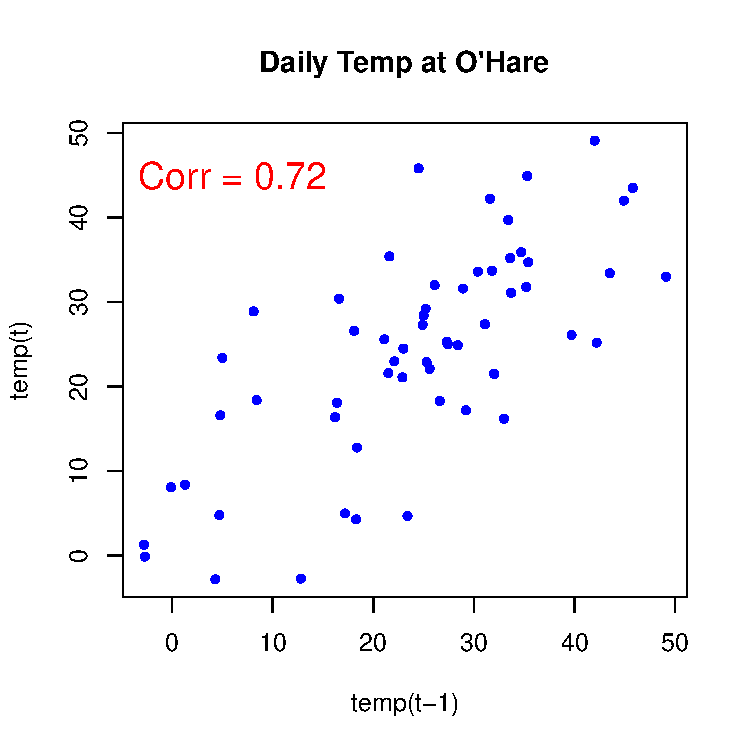
\includegraphics[scale=0.5,trim=20 30 0 25]{templast_new}
\end{minipage}
\begin{minipage}{3.75cm}
\begin{itemize}
\item Correlation between $Y_t$ and $Y_{t-1}$ is called {\rd autocorrelation}.
\end{itemize}
\end{minipage}
\end{center}

\vspace{-0.5cm}
\end{frame}


\begin{frame}
\nochap

 We can plot $Y_t$ against $Y_{t-\ell}$ to see {\rd $\ell$-period lagged relationships}.
\begin{center}
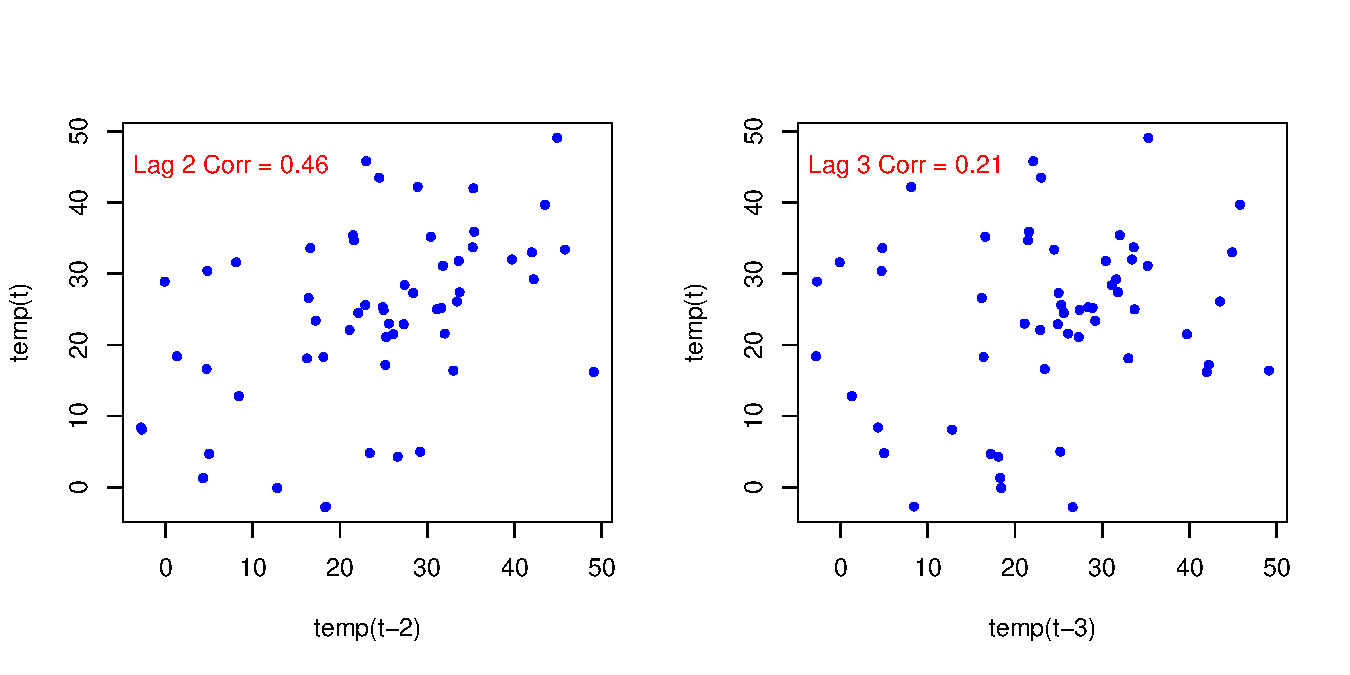
\includegraphics[scale=0.5,trim=10 25 0 70]{lagtemp_new}
\end{center}

\begin{itemize}
\item It appears that the correlation is getting weaker with increasing $\ell$.
\end{itemize}

\end{frame}


\begin{frame}[fragile]
\chap{Autocorrelation}

To summarize the time-varying dependence, compute lag-$\ell$ correlations for
$\ell=1,2,3,\ldots$

\sk
In general, the autocorrelation function (ACF) for $Y$ is
\[\rd
r(\ell) = \mr{cor}(Y_t, Y_{t-\ell})
\]

\vspace{-0.55cm}
For our O'Hare temperature data:

{\footnotesize \bl 
\begin{verbatim}
> print(acf(weather$temp)) 
    0     1     2     3     4     5     6     7     8 
 1.00  0.71  0.44  0.20  0.07  0.09  0.04 -0.01 -0.09 
    9    10    11    12    13    14    15    16    17 
-0.10 -0.07  0.03  0.05 -0.01 -0.06 -0.06  0.00  0.10 
\end{verbatim}
}

\nsk
\end{frame}

\begin{frame}
\nochap

\vspace{-0.35cm}
R's \R{acf} function shows the ACF visually.

\begin{center}
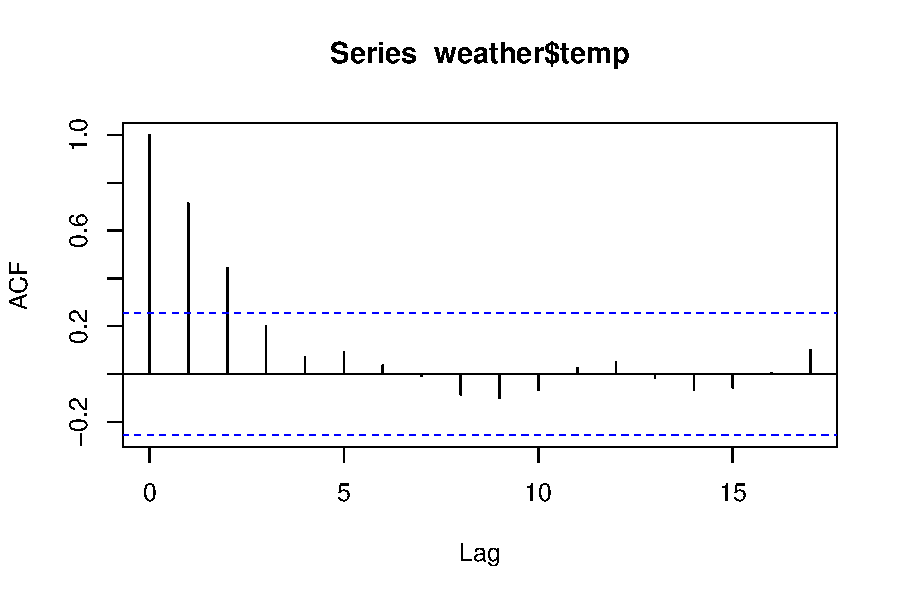
\includegraphics[scale=0.62,trim=10 25 0 20]{tempacf_new}
\end{center}

It provides a visual summary of our data dependence.\\
{\small \hfill ({\bl Blue lines mark ``statistical significance'' for the {\tt acf} values.})}
\end{frame}



\begin{frame}
\nochap

The acf plot for the {\fg beer data} shows an alternating dependence
structure which causes time series oscillations.

\begin{center}
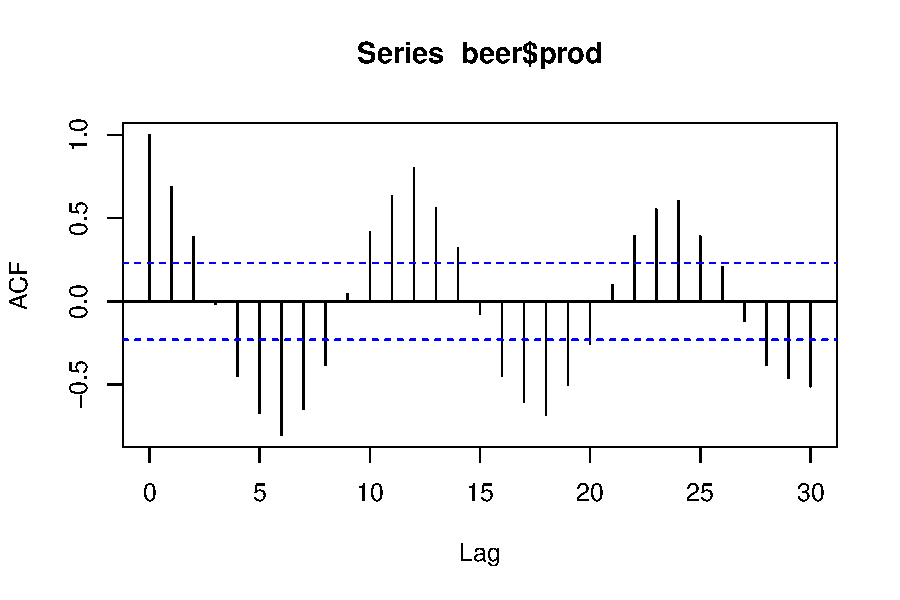
\includegraphics[scale=0.68,trim=10 25 0 15]{beeracf_new}
\end{center}

\end{frame}

\begin{frame}
\nochap

An acf plot for {\fg $iid$ normal data} shows no significant correlation.

\begin{center}
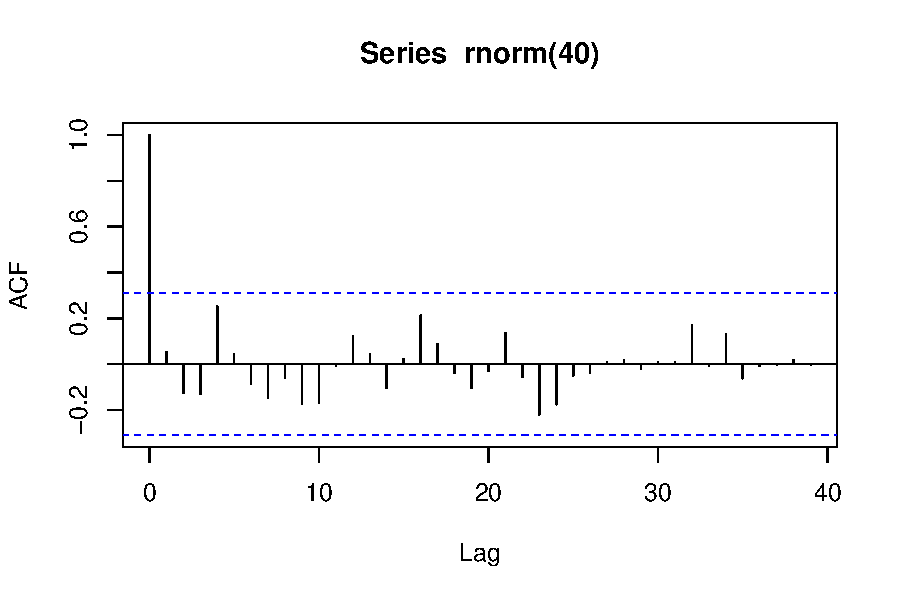
\includegraphics[scale=0.68,trim=10 25 0 15]{normacf_new}
\end{center}

\end{frame}


\begin{frame}
\chap{Autoregression}

{\bl How do we model data that exhibits autocorrelation?}

\sk 
Suppose $Y_1 = \varepsilon_1$, $Y_2 = \varepsilon_{1} +
\varepsilon_{2}$, $Y_3 = \varepsilon_{1} + \varepsilon_{2} +
\varepsilon_{3}$, etc.

\begin{center}
\bl Then 
$Y_t =  \sum_{i=1}^{t}\varepsilon_i = Y_{t-1} + \varepsilon_t$ and $\E[Y_t] = Y_{t-1}$.
\end{center}

\vspace{0.1cm}
This is called a {\rd random walk} model for $Y_t$: 
\begin{itemize}
\item the expectation of what will happen is always what happened most recently.
\end{itemize}

\sk
Even though $Y_t$ is a function of errors going all the way back to the 
beginning, you can write it as depending only on $Y_{t-1}$.
\end{frame}

\begin{frame}
\nochap

Random walks are just a version of a more general model ...

\sk
The {\bl autoregressive} model of order one holds that
\[
\rd AR(1): Y_t = \beta_0 + \beta_1Y_{t-1} + \varepsilon_t,
 \;\;\; \varepsilon_t \stackrel{\mathrm{iid}}{\sim}\mN(0, \sigma^2).
\]
{\fg This is just a SLR model of $Y_t$ regressed onto lagged $Y_{t-1}$.}

\sk It assumes all of our standard regression model conditions.

\begin{itemize}
\item The residuals should look $iid$ and be uncorrelated with $\hat{Y}_t$.
\item All of our previous diagnostics and transforms still apply.
\end{itemize}

\end{frame}

\begin{frame}
\nochap

{\large \[
\rd AR(1): Y_t = \beta_0 + \beta_1Y_{t-1} + \varepsilon_t
\]}
\vskip -.25cm
Again, $Y_t$ depends on the past only
through $Y_{t-1}$.  
\begin{itemize} 
\item {\bl Previous lag values ($Y_{t-2}, Y_{t-3},\ldots$) do not help 
predict $Y_t$ if you already know $Y_{t-1}$.}
\end{itemize}

\sk
Think about daily temperatures:  
\begin{itemize}
\item If I want to guess tomorrow's 
temperature (without the help of a meterologist!), it is 
sensible to base my prediction on today's temperature, ignoring yesterday's.
\end{itemize}
\end{frame}

\begin{frame}[fragile]
\nochap

\vspace{-0.2cm}
For the O'Hare temperatures, there is a clear autocorrelation.

{\bl \footnotesize
\begin{verbatim}
> tempreg <- lm(weather$temp[2:59] ~ weather$temp[1:58])
> summary(tempreg)  ## abbreviated output

Coefficients:
                   Estimate Std. Error t value Pr(>|t|)    
(Intercept)         6.70580    2.51661   2.665   0.0101 *  
weather$temp[1:58]  0.72329    0.09242   7.826  1.5e-10 ***
---
Signif. codes:  0 ‘***’ 0.001 ‘**’ 0.01 ‘*’ 0.05 ‘.’ 0.1 ‘ ’ 1

Residual standard error: 8.79 on 56 degrees of freedom
Multiple R-squared:  0.5224,  Adjusted R-squared:  0.5138 
F-statistic: 61.24 on 1 and 56 DF,  p-value: 1.497e-10
\end{verbatim}
}

\vspace{-0.25cm}
\begin{itemize}
\item The autoregressive term ($b_1 \approx 0.7$) is highly significant!
\end{itemize}

\end{frame}


\begin{frame}[fragile]
\nochap

We can check residuals for any ``left-over'' correlation.

{\bl
\begin{verbatim}
> acf(tempreg$residuals)
\end{verbatim}
}

\begin{center} 
\begin{minipage}{7.5cm}
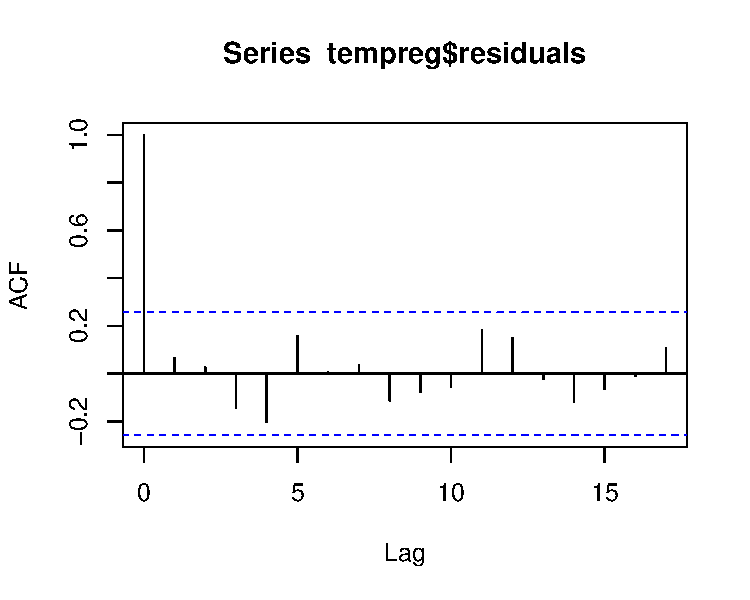
\includegraphics[scale=0.68,trim=15 25 0 20]{acftempreg_new}
\end{minipage}
\begin{minipage}{3cm}
\begin{itemize}
\item Looks like we've got a good fit.
\end{itemize}
\end{minipage}
\end{center}

\end{frame}


\begin{frame}[fragile]
\nochap

For the beer data, the autoregressive term is also highly significant.

{\bl \footnotesize
\begin{verbatim}
> beerreg <- lm(beer$prod[2:72] ~  beer$prod[1:71])
> summary(beerreg) ## abbreviated output

Coefficients:
                Estimate Std. Error t value Pr(>|t|)    
(Intercept)     10.64818    3.56983   2.983  0.00395 ** 
beer$prod[1:71]  0.69960    0.08748   7.997 2.02e-11 ***
---
Signif. codes:  0 ‘***’ 0.001 ‘**’ 0.01 ‘*’ 0.05 ‘.’ 0.1 ‘ ’ 1

Residual standard error: 14.08 on 69 degrees of freedom
Multiple R-squared:  0.481, Adjusted R-squared:  0.4735 
F-statistic: 63.95 on 1 and 69 DF,  p-value: 2.025e-11
\end{verbatim}
}

\end{frame}

\begin{frame}[fragile]
\nochap

But residuals show a clear pattern of left-over autocorrelation.
{\bl
\begin{verbatim}
> acf(beerreg$residuals)
\end{verbatim}
}

\begin{center} 
\begin{minipage}{7.5cm}
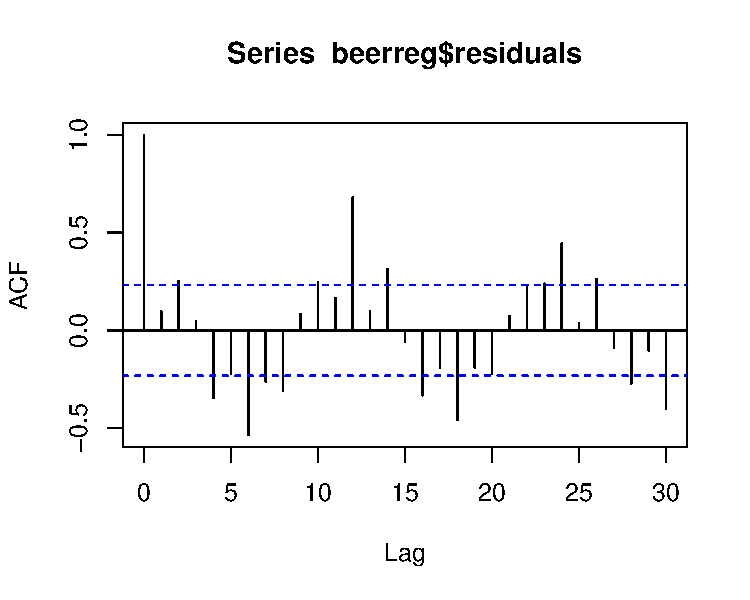
\includegraphics[scale=0.68,trim=15 25 0 20]{acfbeerreg_new}
\end{minipage}
\begin{minipage}{3cm}
\begin{itemize}
\item We'll talk later about how to model this type of pattern ...
\end{itemize}
\end{minipage}
\end{center}

\end{frame}


\begin{frame}
\nochap

Many different types of series may be written as an AR$(1)$.
\[
AR(1): Y_t = \beta_0 + \beta_1Y_{t-1} + \varepsilon_t
\]

{\bl The value of $\beta_1$ is key!}
\begin{itemize}
\item If $|\beta_1| = 1$, we have a {\em random walk}.
\item If $|\beta_1| > 1$, the series {\em explodes}.
\item If $|\beta_1| < 1$, the values are {\em mean reverting}.
\end{itemize}

\end{frame}

\begin{frame}
\chap{Random walk}

In a random walk, the series just wanders around.
\begin{center}
\ \ $\beta_1 = 1$\\
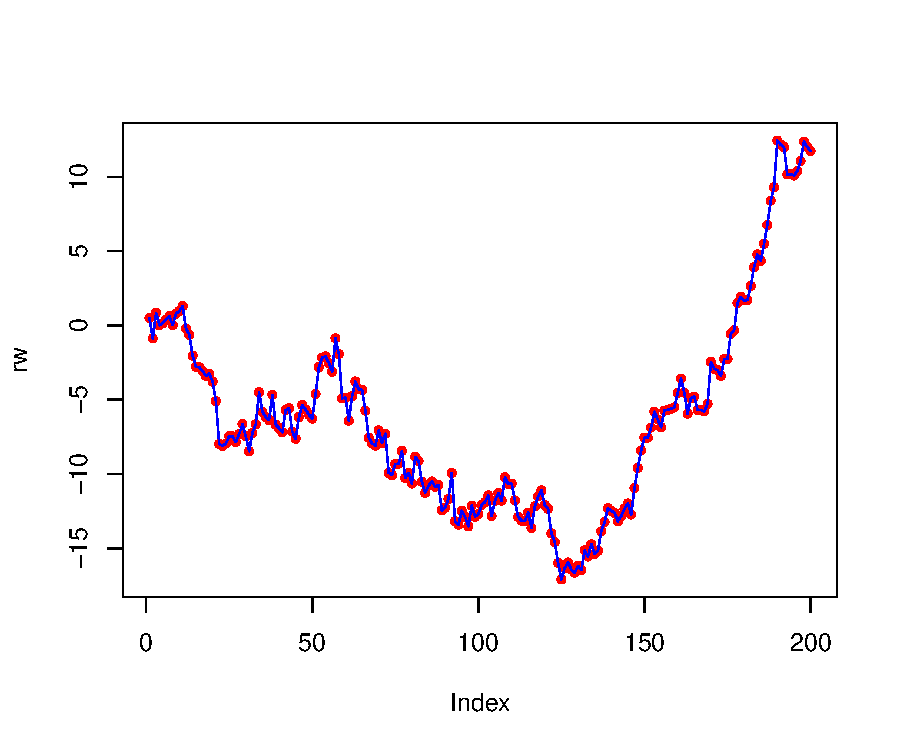
\includegraphics[scale=0.55,trim=10 50 0 50]{randwalk_new}
\end{center}

\end{frame}

\begin{frame}
\nochap

Autocorrelation of a random walk stays high for a long time.

\begin{center}
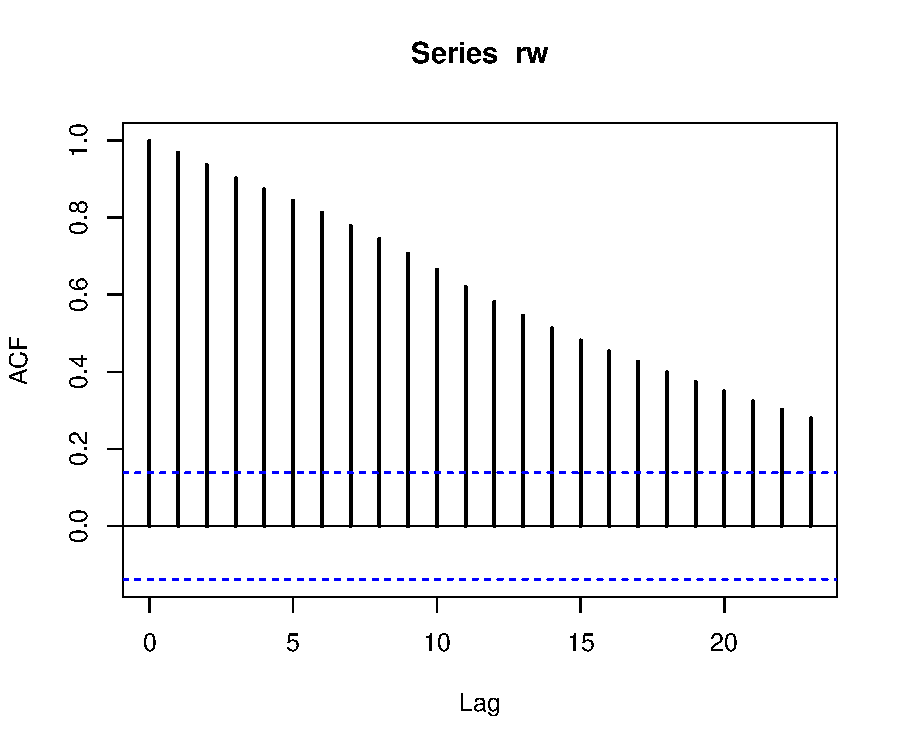
\includegraphics[scale=0.55,trim=20 20 0 10]{acfrandwalk_new}
\end{center}

\end{frame}


\begin{frame}
\nochap

The random walk has some special properties ...

\sk
$\bl Y_t - Y_{t-1} = \beta_0 + \varepsilon_t$, 
and $\beta_0$ is called the ``drift parameter''.

\sk
The series is {\bl nonstationary}: 
\begin{itemize}
\item it has no average level that it wants to be near, 
but rather just wanders off into space.
\end{itemize}

\sk 
The random walk {\rd without drift ($\beta_0 = 0$)} is a common model for
simple processes
\begin{itemize}
\item since {\bl $\E[Y_t] = \E[Y_{t-1}]$}, e.g., tomorrow $\approx$
today
\end{itemize}

\end{frame}

\iffalse
\begin{frame}
\nochap

{\bl Example:} monthly Dow Jones composite index, 2000--2007.

\begin{center}
\includegraphics[scale=0.55,trim=20 40 0 50]{dja_new}
\end{center}
\begin{itemize}
\item Appears as though it is just wandering around.
\end{itemize}
\end{frame}


\begin{frame}[fragile]
\nochap

Sure enough, our regression indicates a random walk ($b_1 \approx 1$):

{\bl \footnotesize
\begin{verbatim}
> n <- length(dja)
> ARdj <- lm(dja[2:n] ~ dja[1:(n-1)])
> summary(ARdj)  ## abbreviated output

Coefficients:
               Estimate Std. Error t value Pr(>|t|)    
(Intercept)     7.05419    4.00385   1.762   0.0782 .  
dja[1:(n - 1)]  0.99764    0.00121 824.298   <2e-16 ***
---
Signif. codes:  0 ‘***’ 0.001 ‘**’ 0.01 ‘*’ 0.05 ‘.’ 0.1 ‘ ’ 1
\end{verbatim}
}

\begin{itemize}
\item $b_0 > 0$, but not enough data to be {\rd sure} of positive drift.
\end{itemize}
\end{frame}



\begin{frame}[fragile]
\nochap

When you switch to returns, however, it's just white noise.

{\bl \scriptsize
\begin{verbatim}
> returns <- (dja[2:n]-dja[1:(n-1)])/dja[1:(n-1)]
> plot(returns, type="l", col=3, xlab="day", ylab="DJA Return")
\end{verbatim}
}

\begin{center}
\includegraphics[scale=0.6,trim=20 35 0 55]{return_new}
\end{center}

\vspace{-0.1cm}
\begin{itemize}
\item $(Y_t - Y_{t-1})/Y_{t-1}$ appears to remove the dependence.
\end{itemize}

\end{frame}

\begin{frame}[fragile]
\nochap

\vspace{-0.25cm}
And now the regression model finds nothing significant.

{\bl \footnotesize
\begin{verbatim}
> ret <- lm(returns[2:n] ~ returns[1:(n-1)])
> summary(ret) ## abbreviated output

Coefficients:
                     Estimate Std. Error t value Pr(>|t|)
(Intercept)        -0.0001138  0.0002363  -0.482    0.630
returns[1:(n - 1)] -0.0144411  0.0225321  -0.641    0.522

Residual standard error: 0.01051 on 1975 degrees of freedom
  (1 observation deleted due to missingness)
Multiple R-squared: 0.000208, Adjusted R-squared: -0.000298 
F-statistic: 0.4108 on 1 and 1975 DF,  p-value: 0.5217
\end{verbatim}
}

This is common with random walks: {\rd $Y_{t}- Y_{t-1}$ is iid}.
\end{frame}
\fi

\begin{frame}
\chap{Exploding series}

For AR term $>1$, the $Y_t$'s move exponentially far from $Y_1$.

\vspace{0.55cm}
\begin{minipage}{7cm}
\centering
\ \ \ \ \ \ \ \ \ \ \ $\beta_1 = 1.02$\\
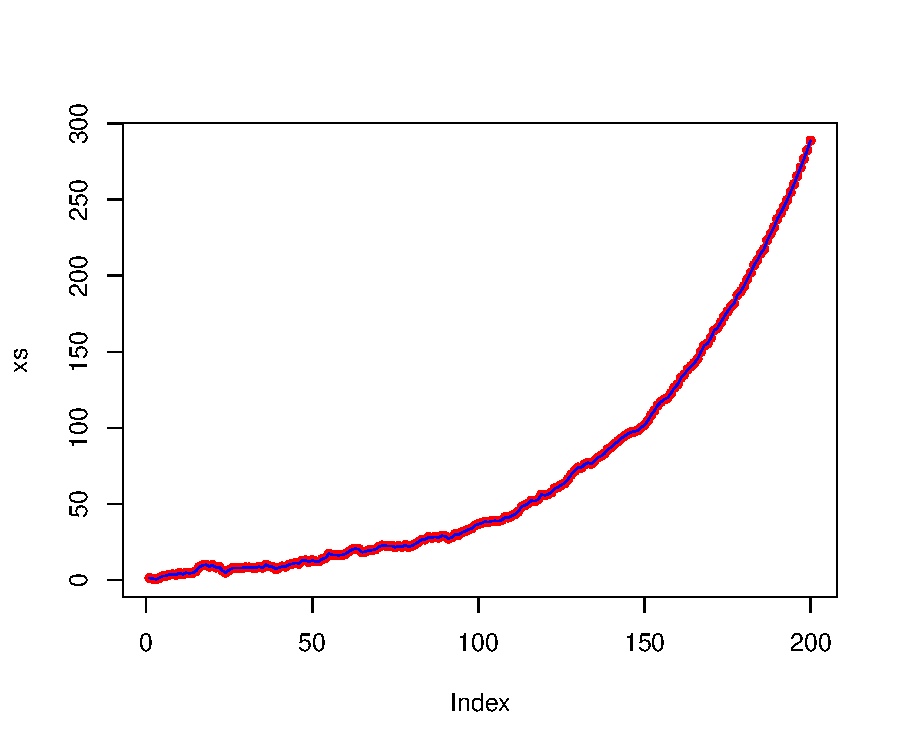
\includegraphics[scale=0.55,trim=15 50 0 50]{exploding_new}
\sk
\end{minipage}\hfill
\begin{minipage}{3cm}
\begin{itemize}
\item Useless for modeling and prediction.
\end{itemize}
\end{minipage}
\end{frame}


\begin{frame}
\chap{Stationary series}

For AR term $<1$, $Y_t$ is always pulled back towards the mean.

\vspace{0.55cm}
\begin{minipage}{7cm}
\centering
\ \ \ \ \ \ \ \ \ \ \ $\beta_1 = 0.8$\\
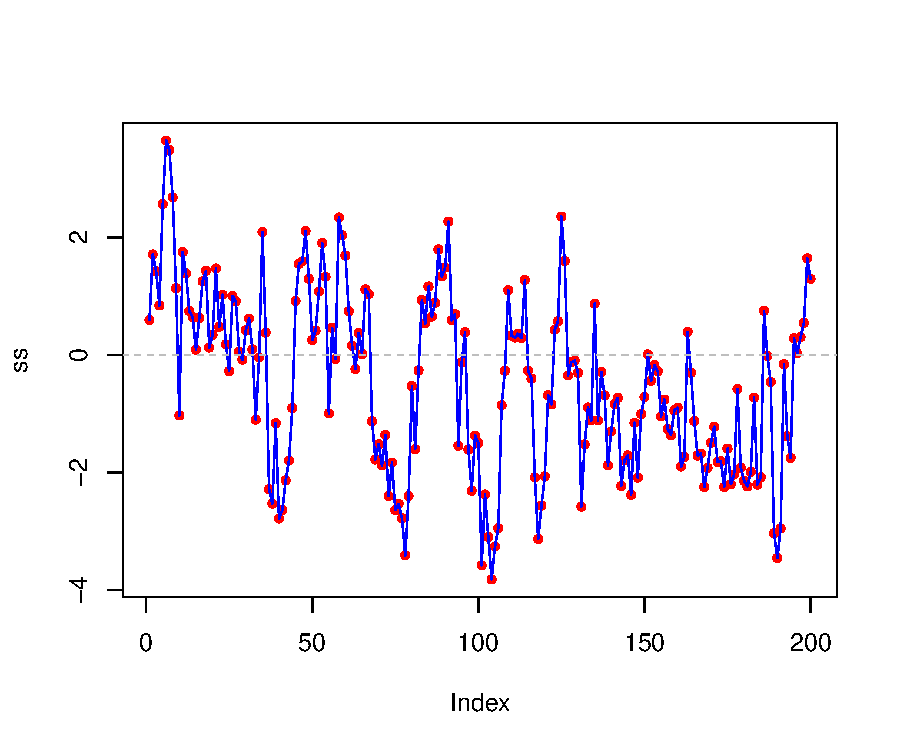
\includegraphics[scale=0.55,trim=15 50 0 50]{stationary_new}
\sk
\end{minipage}\hfill
\begin{minipage}{3cm}
\begin{itemize}
\item These are the most common, and most useful, type of AR series.
\end{itemize}
\end{minipage}

\end{frame}

\begin{frame}
\nochap

Autocorrelation for the stationary series drops off right away.

\vspace{0.55cm}
\begin{minipage}{7cm}
\centering
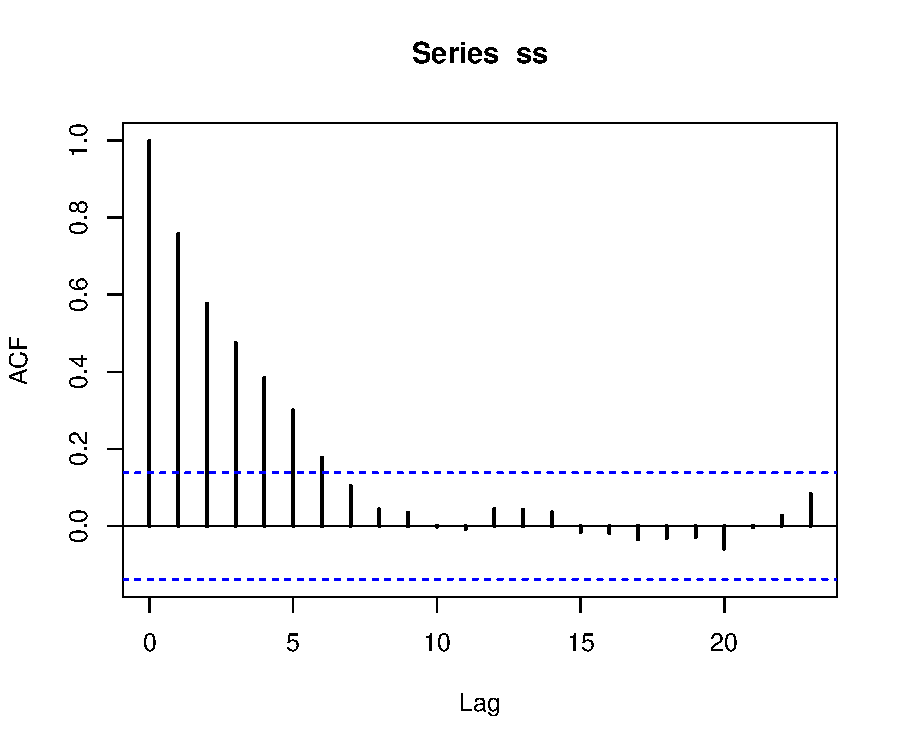
\includegraphics[scale=0.55,trim=15 30 0 10]{acfstationary}
\sk
\end{minipage}\hfill
\begin{minipage}{3cm}
\nsk
\begin{itemize}
\item The past matters, but with limited horizon.
\end{itemize}
\end{minipage}

\end{frame}

\begin{frame}
\chap{Mean reversion}

An important property of stationary series is {\rd mean reversion}.

\sk
Think about shifting both $Y_t$ and $Y_{t-1}$ by their mean $\mu$.
\[ 
\bl Y_t - \mu = \beta_1 (Y_{t-1} - \mu) +\varepsilon_t
\]
Since $|\beta_1| < 1$, $Y_t$ is expected to be closer to $\mu$
than $Y_{t-1}$.

\sk 
Mean reversion is all over, and helps predict
future behaviour:
\begin{itemize}
%\item ``alpha'' in repeated CAPM models,
\item weekly sales numbers,
\item daily temperature.
\end{itemize}

\end{frame}

\begin{frame}
\chap{Negative correlation}

It is also possible to have negatively correlated AR(1) series.

\vspace{0.55cm}
\begin{minipage}{7cm}
\centering
\ \ \ \ \ \ \ \ \ \ \ $\beta_1 = -0.8$\\
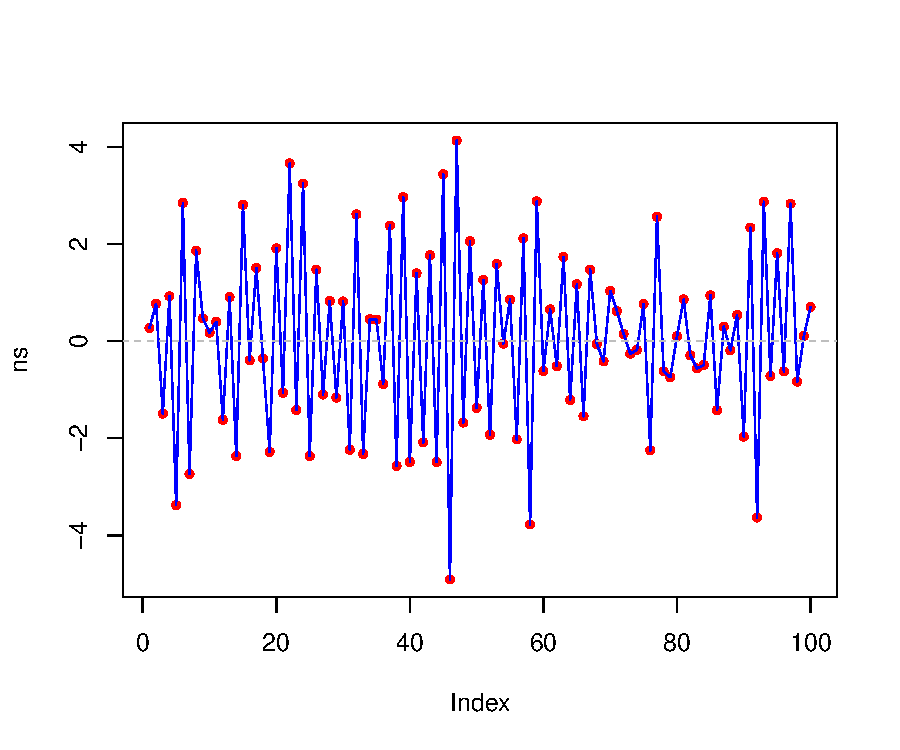
\includegraphics[scale=0.55,trim=15 50 0 50]{negcor_new}
\sk
\end{minipage}\hfill
\begin{minipage}{3cm}
\begin{itemize}
\item But you see these far less often in practice.
\end{itemize}
\end{minipage}

\end{frame}

\begin{frame}
\chap{Summary of AR(1) behavior}

%\small
\vspace{0.25cm}
\hfill \begin{minipage}{10.25cm}
\begin{itemize}
\item[$|\beta_1| < 1$:]
The series has a mean level to which it reverts.  For 
positive $\beta_1$, the series tends to wander above or below 
the mean level for a while.  For negative $\beta_1$, the series 
tends to flip back and forth around the mean. 
The series is stationary, meaning that the 
mean level does not change over time.  
\item[$|\beta_1| = 1$:] A random walk series.
The series has no mean level and, thus, is called 
nonstationary.  The drift parameter $\beta_0$ is the direction in 
which the series wanders.
\item[$|\beta_1| > 1$:] 
The series explodes, is nonstationary, and pretty much useless.
\end{itemize}
\end{minipage}
\end{frame}

\begin{frame}[fragile]
\chap{AR($p$) models}

It is possible to expand the AR idea to higher lags
\[
\rd AR(p): Y_t = \beta_0 + \beta_1Y_{t-1} + \cdots + \beta_pY_{t-p} + \varepsilon.
\]

\vspace{-0.5cm}
For example, a 12 month lag for the beer data:
{\bl \footnotesize
\begin{verbatim}
> beerreg12 <- lm( beer$prod[12:72] ~  beer$prod[1:61])
> summary(beerreg12) ## abbreviated output

Coefficients:
                Estimate Std. Error t value Pr(>|t|)    
(Intercept)     10.25404    3.69629   2.774   0.0074 ** 
beer$prod[1:61]  0.70093    0.09102   7.701 1.75e-10 ***
\end{verbatim}
}
\end{frame}


\begin{frame}
\chap{AR($p$) models}

It is possible to expand the AR idea to higher lags
\[
\rd AR(p): Y_t = \beta_0 + \beta_1Y_{t-1} + \cdots + \beta_pY_{t-p} + \varepsilon.
\]

\vspace{-0.5cm}
However, it is seldom necessary to fit AR lags for $p>1$.
\begin{itemize}
\item Like having polynomial terms higher than 2, this just isn't usually
required in practice.
\item You lose all of the stationary/nonstationary
intuition.
\item Often, the need for higher lags is symptomatic of (missing) a more
persistent trend or periodicity in the data ...
\end{itemize}
\end{frame}



\begin{frame}
\chap{Trending series}

Often, you'll have a linear trend in your time series.
\begin{itemize}
\item[$\Rightarrow$] AR structure, sloping up or down in time.
\end{itemize}

\begin{center}
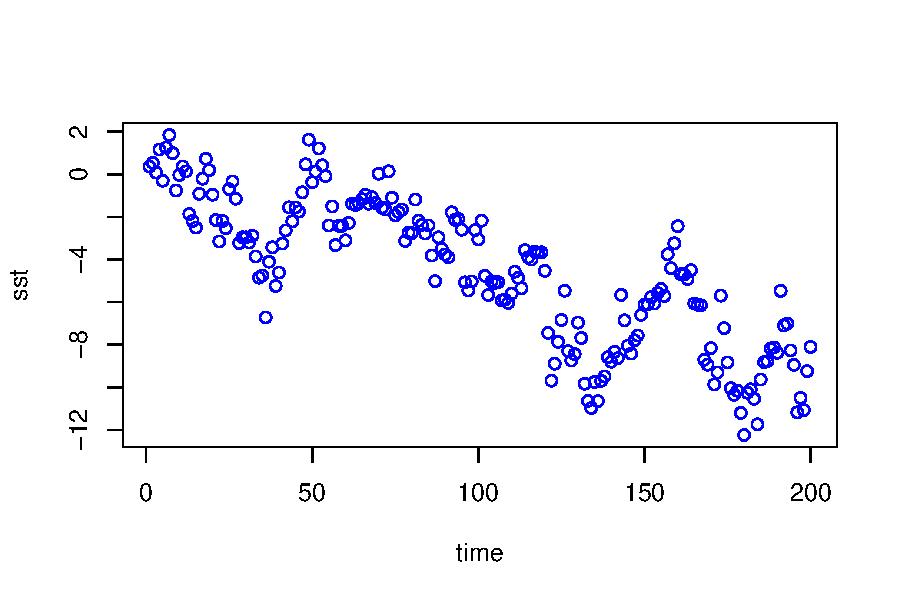
\includegraphics[scale=0.6,trim=15 50 0 50]{artime}
\end{center}

\end{frame}

\begin{frame}[fragile]
\nochap

\vspace{-0.1cm}
This is easy to deal with: just put ``time'' in the model.

\vspace{0.25cm}
AR with linear trend:
\[
\rd Y_t =  \beta_0 + \beta_1Y_{t-1} +
\beta_2t + \varepsilon_t
\]

\vspace{-1cm}
{\bl \small
\begin{verbatim}
> t <- 1:199
> sst.fit <- lm(sst[2:200] ~ sst[1:199] + t)
> summary(sst.fit)  ## abbreviated output

Coefficients:
             Estimate Std. Error t value Pr(>|t|)    
(Intercept) -0.571525   0.178110  -3.209  0.00156 ** 
sst[1:199]   0.735840   0.048062  15.310  < 2e-16 ***
t           -0.009179   0.002160  -4.249 3.32e-05 ***
\end{verbatim}
}
\end{frame}

\begin{frame}
\chap{Periodic models}

It is very common to see {\rd seasonality} or {\rd periodicity} in
series.
\begin{itemize}
\item Temperature goes up in Summer and down in Winter.  
\item Natural gas consumption in London or Chicago would do the opposite.
\end{itemize}

\sk
Recall the monthly beer production data:
\begin{minipage}{6cm}
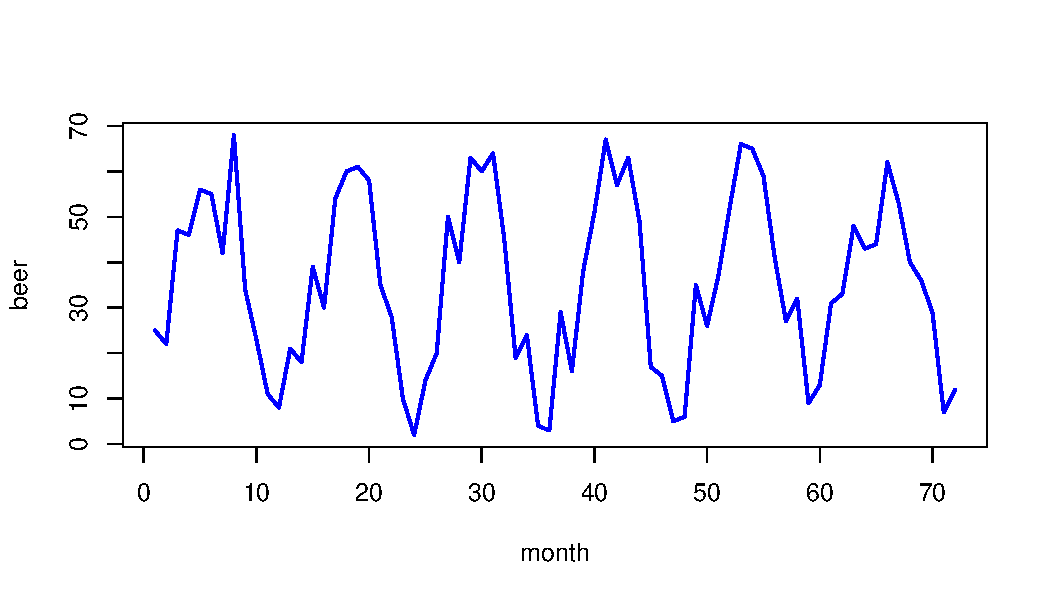
\includegraphics[scale=0.48,trim=10 20 0 25]{beer_new}
\end{minipage} \hfill
\begin{minipage}{2.85cm}
\nsk
\begin{itemize}
\item Appears to oscillate on a 12-month cycle.
\end{itemize}
\end{minipage}
\end{frame}

\begin{frame}
\nochap

\vspace{-0.3cm}
The  straightforward solution:  Add periodic predictors.

\sk
$\mathrm{Period}\!-\!k~\mbox{model}\!:$
\vspace{-0.35cm}
\[
\rd Y_t = \beta_0 + \beta_1\sin(2\pi t /k) + \beta_2\cos(2\pi t /k)
+ \varepsilon_t 
\]

\vspace{-0.5cm}
Remember your {\rd sine} and {\bl cosine}!
\begin{center}
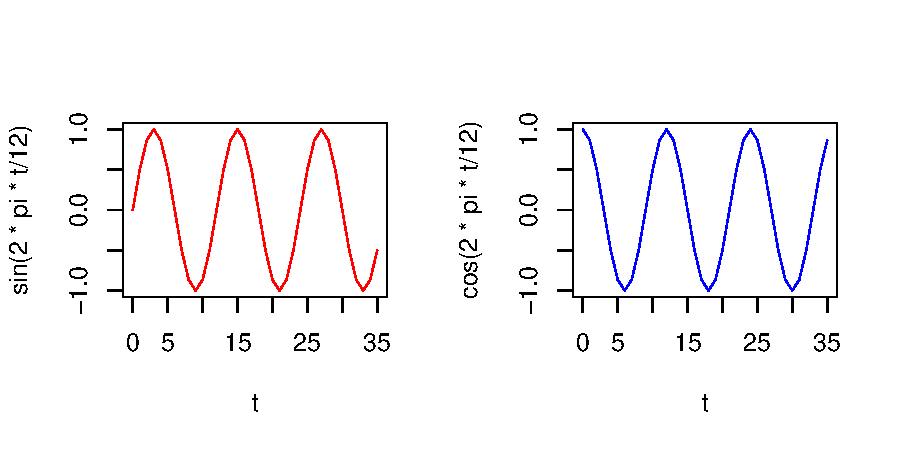
\includegraphics[scale=0.75,trim=0 25 20 70]{sincos_new}
\end{center}

\vspace{-0.25cm}
\begin{itemize}
\item Repeating themselves every $2\pi$.
\end{itemize}

\end{frame}

\begin{frame}
\nochap

$\mathrm{Period}\!-\!k~\mbox{model}\!:$
\vspace{-0.35cm}
\[
\rd Y_t = \beta_0 + \beta_1\sin(2\pi t /k) + \beta_2\cos(2\pi t /k)
+ \varepsilon_t 
\]

\vspace{-0.5cm}
It turns out that you can represent \bl any \bk smooth periodic function 
as a sum of sines and cosines.

\sk
You choose $k$ to be the number of ``times'' in a single period.
\begin{itemize}
\item For monthly data, $k = 12$ implies an annual cycle.
\item For quarterly data, usually $k=4$.
\item For hourly data, $k=24$ gives you a daily cycle.
\end{itemize}

\end{frame}

\begin{frame}
\nochap

\vspace{-0.15cm}
{\bl Putting it all together:} Airline data
\begin{itemize}
\item $Y_t = $ monthly total international passengers, 1949-1960.
\end{itemize}

\begin{center}
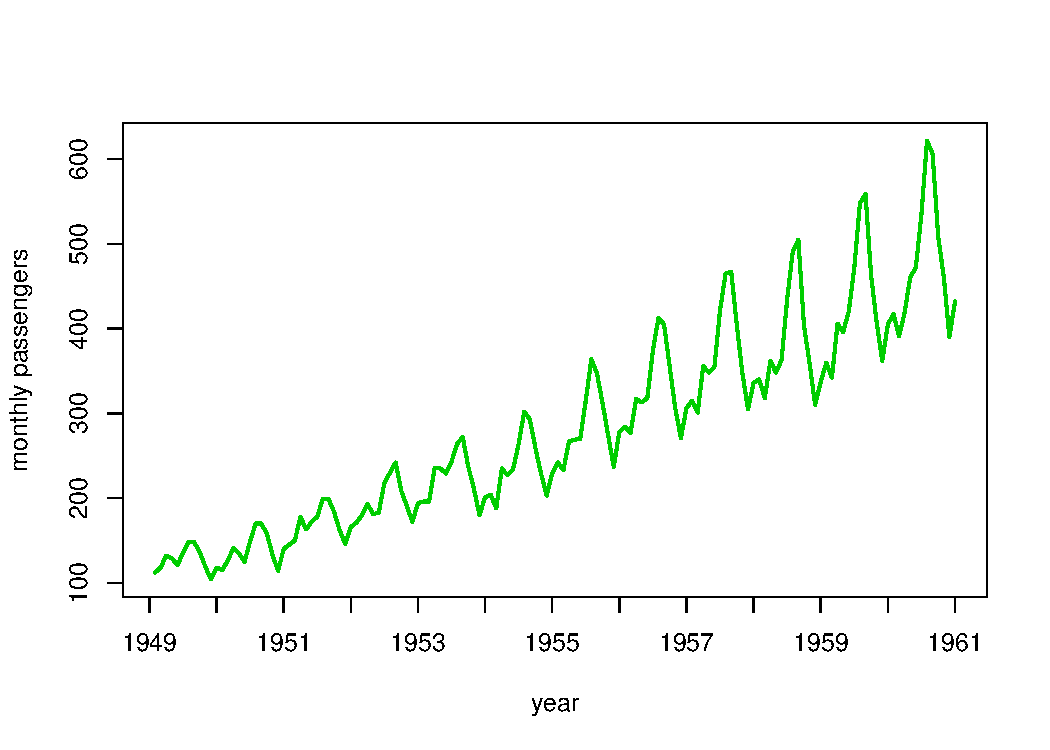
\includegraphics[scale=0.5,trim=10 20 0 60]{airline_new}
\end{center}

\nsk
\begin{itemize}
\item  {\bl What do you notice in the data?} % Increasing annual oscillation and positive linear trend.
\end{itemize}

\end{frame}

\begin{frame}
\nochap

\vspace{-0.15cm}
The data shows a strong persistence in correlation.

\begin{center}
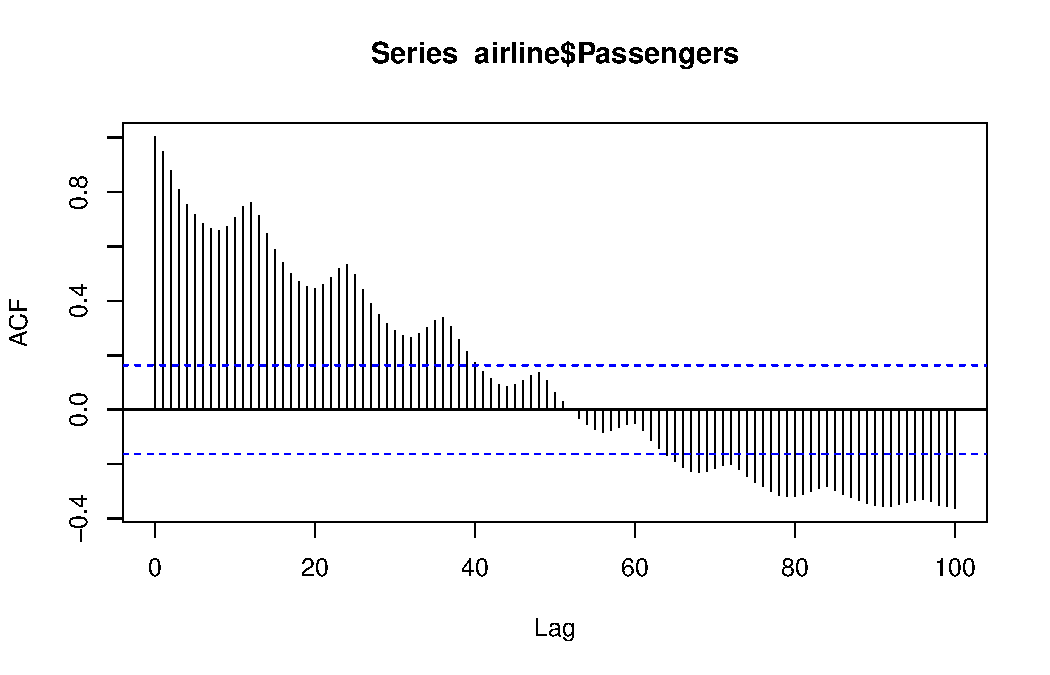
\includegraphics[scale=0.55,trim=10 20 0 20]{airlineacf_new}
\end{center}

\vspace{-0.15cm}
Annual (12 month) periodicity shows up here as well.

\end{frame}

\begin{frame}
\nochap

\vspace{-0.1cm}
Fitting the model: first, don't forget your fundamentals!
\begin{itemize}
\item The series variance is increasing in time.
%\item Passenger numbers are like sales volume.
\item {\rd We need to work on log/sqrt scale!}
\end{itemize}

\begin{center}
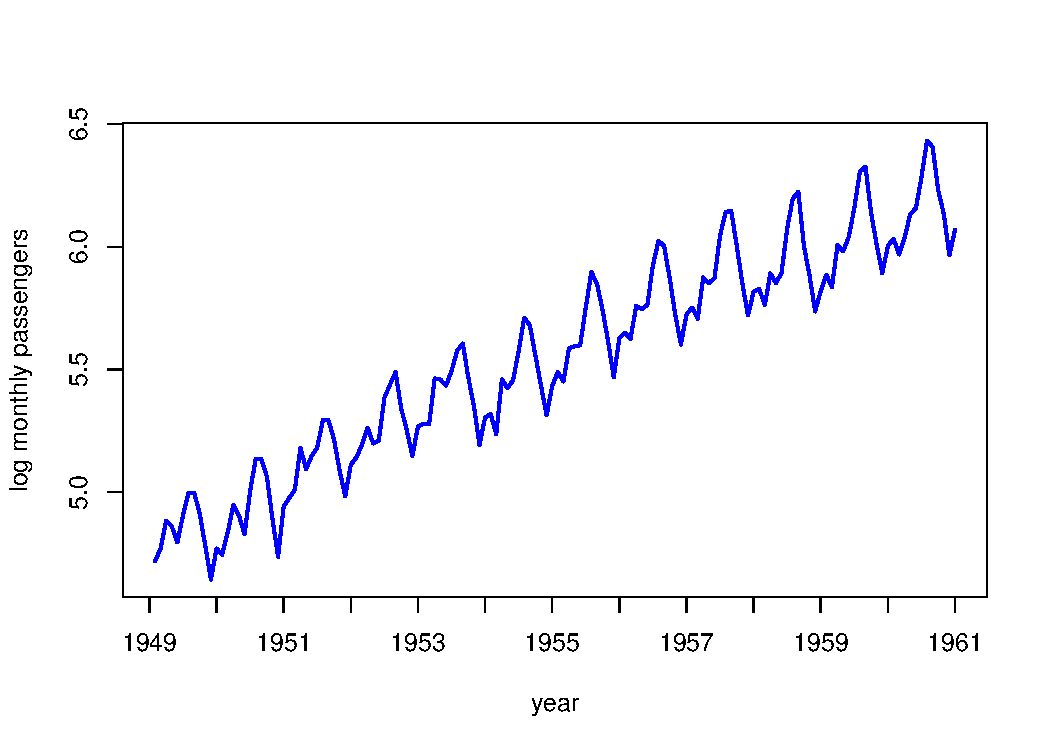
\includegraphics[scale=0.5,trim=10 20 0 50]{logairline_new}
\end{center}

\end{frame}

\begin{frame}[fragile]
\nochap

The series shows a linear trend, an oscillation of period 12, 
and we expect to find autoregressive errors.  

\nsk
{\rd 
\begin{align*}
\log(Y_t) &= \beta_0 + \beta_1 \log(Y_{t-1}) + \beta_2t \\
&\;\;\; + \beta_3\sin\left(\frac{2\pi t }{12}\right) + \beta_4\cos\left(\frac{2\pi t }{12}\right)
+ \varepsilon_t 
\end{align*}
}

\sk
You'll practice with this dataset a little later.
%Open the {\tt \bl VB\_TS\_exercise.Rmd} file, and start fitting some TS models.

%\nsk
%{\bl \footnotesize
%\begin{verbatim}
%> t <- 2:nrow(airline)
%> YX <- data.frame(logY=log(airline$Passengers[2:144]),
%+   logYpast=log(airline$Passengers[1:143]), t=t,
%+   sin12=sin(2*pi*t/12), cos12=cos(2*pi*t/12))
%> airlm <- lm(logY ~ logYpast + t + sin12 + cos12, data=YX)
%\end{verbatim}
%}

\end{frame}


%%%%%%%%%%%%%%%%%%%%%%%%%%%%%%%%%%%%%%%%%%%%%%%%%%
%%%%%%%%%%%%%%%%%%%%%%%%%%%%%%%%%%%%%%%%%%%%%%%%%%

\iffalse 
\begin{frame}[fragile]
\nochap

\vspace{-0.25cm}
{\bl \footnotesize
\begin{verbatim}
> summary(airlm) ## abbreviated output

Coefficients:
              Estimate Std. Error t value Pr(>|t|)    
(Intercept)  2.5323909  0.3603010   7.029 8.77e-11 ***
logYpast     0.4748286  0.0749506   6.335 3.12e-09 ***
t            0.0052759  0.0007703   6.849 2.25e-10 ***
sin12        0.0040818  0.0126512   0.323    0.747    
cos12       -0.0960295  0.0119032  -8.068 3.12e-13 ***
---
Signif. codes:  0 ‘***’ 0.001 ‘**’ 0.01 ‘*’ 0.05 ‘.’ 0.1 ‘ ’ 1

Residual standard error: 0.07929 on 138 degrees of freedom
Multiple R-squared:  0.9681,  Adjusted R-squared:  0.9672 
F-statistic:  1047 on 4 and 138 DF,  p-value: < 2.2e-16
\end{verbatim}
}

\end{frame}

\begin{frame}
\nochap

\vspace{-0.35cm}
The model predictions look pretty good!
\begin{center}
\includegraphics[scale=0.58,trim=10 10 0 50]{airpred_new}
\end{center}

\nsk
\begin{itemize}
\item Sine and cosine trends seem to capture the periodicity.
\end{itemize}

\end{frame}


\begin{frame}
\nochap

\vspace{-0.15cm}
However, a closer look exposes residual autocorrellation.

\begin{center}
\includegraphics[scale=0.68,trim=20 5 0 35]{airresid_new}
\end{center}

\nsk
\hfill \begin{minipage}{5cm}
\begin{itemize}
\item {\rd How can we fix this?}
\end{itemize}
\end{minipage}

\end{frame}


\begin{frame}
\nochap

\vspace{-0.25cm}
You can see the relationship show up in monthly residuals.
\begin{center}
\includegraphics[scale=0.58,trim=10 10 0 50]{airmonths_new}
\end{center}
\nsk
\begin{itemize}
\item This is probably due to holiday/shoulder season effects.
\end{itemize}
\end{frame}

\begin{frame}[fragile]
\nochap

We create some useful dummy variables:
{\bl \small
\begin{verbatim}
> YX$holidays <- airline$Month[t] %in% c(3,6,7,8,12) 
> YX$jan <- airline$Month[t]==1
> YX$nov <- airline$Month[t]==11
> YX$jul <- airline$Month[t]==7
\end{verbatim}
}

\sk
Then re-fit the model with {\tt holidays}, {\tt nov}, {\tt jan}, and {\tt
  jul}.
\begin{itemize}
\item Months with {\tt\rd holidays} have an obvious effect.
\item {\tt\rd nov} and {\tt\rd jan} have fewer vacation days.
\item {\tt\rd jul} is unique as the entire month is school holiday.
\end{itemize}

\end{frame}

\begin{frame}[fragile]
\nochap

\vspace{-0.15cm}
Everything shows up as being very significant.

{\bl \footnotesize
\begin{verbatim}
> airlm2 <- lm(logY ~ logYpast + t + sin12 + cos12
+   + holidays + nov + jan + jul, data=YX)
> summary(airlm2)

Coefficients:
               Estimate Std. Error t value Pr(>|t|)    
(Intercept)   1.3427507  0.1945587   6.902 1.86e-10 ***
logYpast      0.7100231  0.0401417  17.688  < 2e-16 ***
t             0.0028983  0.0004111   7.050 8.57e-11 ***
sin12         0.0332607  0.0069795   4.765 4.84e-06 ***
cos12        -0.0355395  0.0070772  -5.022 1.60e-06 ***
holidaysTRUE  0.1361014  0.0079670  17.083  < 2e-16 ***
novTRUE      -0.0571301  0.0136937  -4.172 5.39e-05 ***
janTRUE       0.0619620  0.0136601   4.536 1.26e-05 ***
julTRUE       0.0473444  0.0131525   3.600 0.000447 ***
\end{verbatim}
}

\end{frame}

\begin{frame}
\nochap

\vspace{-0.15cm}
The one-step-ahead model predictions look even better.
\begin{center}
\includegraphics[scale=0.58,trim=10 10 0 50]{airpred2_new}
\end{center}

\nsk
\begin{itemize}
\item We're now really able to capture the annual dynamics.
\end{itemize}

\end{frame}

\begin{frame}
\nochap

\nsk
\begin{center}
\includegraphics[scale=0.68,trim=20 5 0 35]{airresid2_new}
\end{center}

\nsk
\begin{itemize}
\item There is a bit of left-over 12 month autocorrelation, 
but nothing to get overly worried about.
\end{itemize}

\end{frame}


\begin{frame}
\chap{Alternative Periodicity}

\sk
An alternative way to add periodicity would be to simply add
a dummy variable for each month ({\tt \bl feb, mar, apr, ...}).

\sk
\begin{itemize}
\item This achieves basically the same fit as above, without requiring you to
add sine or cosine.
\item However, this takes 11 periodic parameters while we use
only 6 ({\rd sine} and {\rd cosine} + {\tt\bl holidays}, {\tt\bl nov}, 
{\tt\bl jan}, and {\tt\bl jul}).  
\end{itemize}
\end{frame}

\begin{frame}
\nochap


I like to think of the periodicity as a smooth oscillation, 
with sharp day/month effects
added for special circumstances.

\sk
\begin{itemize}
\item Requires more thought, but leads to better models.
\item The $\sin+\cos$ technique works regardless of the 
number of increments in a period (e.g. 365 days).
\end{itemize}

\sk\sk {\rd The exception:} 
\begin{itemize}
\item Since quarterly data has a period of only 4,
it is often fine to just add ``quarter'' effects.
\end{itemize}
\end{frame}



\begin{frame}
\chap{Time series}

There are many possible models; you can use BIC with 
  \R{extractAIC(reg, k=log(n))} to compare and
choose.
\begin{itemize}
\item (I calculated many BICs to choose the airline month effects.)
\end{itemize}

\sk
The tools here are good, but not the best:
\begin{itemize}
\item In many situations you want to allow for $\beta$ or $\sigma$
parameters that can change in time.
\item This can leave us with some left-over autocorrelation.
\item Classes dedicated to Time Series are offered in the Math/Stats department, which introduce more advanced methods. 
\end{itemize}



\end{frame}

\fi


\end{document}